\documentclass[conference,a4paper]{IEEEtran}

\usepackage[T1]{fontenc}
\usepackage[utf8]{inputenc}
\usepackage{lmodern}
\usepackage{textcomp}
\usepackage{amsmath}
\usepackage{booktabs}
\usepackage{multirow}
\usepackage{xcolor}
\usepackage{listings}
\usepackage{tikz}
\usetikzlibrary{arrows.meta,positioning,calc}
\usepackage{pgfplots}
\pgfplotsset{compat=1.17}
\usepackage[hyphens]{url}
\usepackage[hidelinks]{hyperref}
\usepackage{cite}

% Allow long identifiers such as keyless_registry() to break at underscores.
\makeatletter
\g@addto@macro{\UrlBreaks}{\do\_\do\.\do\(\do\)}
\makeatother
\DeclareUrlCommand\code{\urlstyle{tt}}
\newcommand{\tbf}{\textbf{[TO BE FILLED]}}
\newcommand{\prov}{provisional}

\lstset{
  basicstyle=\ttfamily\scriptsize,
  columns=fullflexible,
  keepspaces=true,
  breaklines=true,
  breakatwhitespace=false,
  frame=single,
  framesep=2pt,
  xleftmargin=3pt,
  xrightmargin=3pt,
  showstringspaces=false,
  upquote=true,
  literate={°}{\textdegree}1 {–}{--}1
}

\emergencystretch=1.5em

% Start a new, centred row of author blocks.
\makeatletter
\newcommand{\linebreakand}{%
  \end{@IEEEauthorhalign}\hfill\mbox{}\par
  \mbox{}\hfill\begin{@IEEEauthorhalign}}
\makeatother

\begin{document}

\title{ToolAgent: A Small-Scale, DFSDT-Inspired\\ Tool-Use Agent Built After ToolLLM}

\author{
\IEEEauthorblockN{Ayush Mathur}
\IEEEauthorblockA{Student ID: 202411013}
\and
\IEEEauthorblockN{Rudra Mandloi}
\IEEEauthorblockA{Student ID: 202411082}
\and
\IEEEauthorblockN{Yuvank Goyal}
\IEEEauthorblockA{Student ID: 202411100}
\linebreakand
\IEEEauthorblockA{Department of Computer Science / Information Technology\\
Academic Project, Phase 1, 2026}
}

\maketitle

\begin{abstract}
ToolLLM showed how a language model can be taught to pick and call real
web APIs, and how a tree search over reasoning steps (DFSDT) helps on
harder multi-tool tasks~\cite{qin2024toolllm}. In Phase~1 we rebuilt the
main pieces at a size a student team can run on a laptop: a registry of
11 tool wrappers (3 offline mocks and 8 public web APIs), a retriever with
TF-IDF, sentence-embedding and keyword back ends, a ReAct agent, a
DFSDT-inspired agent with depth~4 and breadth~3, an LLM-as-judge
evaluator, and a Streamlit interface. On our own 19-instruction benchmark
the ReAct agent scored 89\% and the DFSDT-inspired agent 84\%. These numbers
are \prov{}: reading the results showed that in 37 of 38 runs the model
wrote the whole episode, including invented tool outputs, in a single
reply, and our loop accepted it. We describe this bug, three argument-parsing
bugs and a retrieval weakness, and how we fixed them with 20 new tests. The
benchmark has not yet been re-run with the fixed code.
\end{abstract}

\begin{IEEEkeywords}
tool use, language model agents, ReAct, depth-first search, API retrieval
\end{IEEEkeywords}

\section{Introduction}

Our project, which we call ToolAgent, asks a simple question: if a
language model can call tools, what does it take to make it pick the
right tool, call it with the right arguments, and give an answer based
on what the tool actually returned? The ToolLLM paper answers this at a
very large scale~\cite{qin2024toolllm}. We cannot repeat that work, so we
built a small version of each part and wired them together ourselves.

The code is split into four Python packages: \code{apis/} (tools),
\code{retriever/} (choosing candidate tools), \code{agent/} (the reasoning
loops and model back ends) and \code{eval/} (judging and reports). A
Streamlit app (\code{app.py}) and three scripts sit on top. In total the
repository holds about 3{,}450 lines of Python, of which 689 are the UI
and 795 are tests.

Our contributions in Phase~1 are:
\begin{itemize}
  \item a uniform \code{BaseAPI} interface and 11 tool wrappers;
  \item three interchangeable retrievers and a small measurement of how
        they rank tools on our benchmark;
  \item a ReAct loop and a DFSDT-inspired search loop that share one
        prompt builder and one action parser;
  \item a benchmark harness with an LLM judge, plus 72 unit tests;
  \item an account of the bugs that made our first benchmark numbers
        unreliable, and the fixes for them.
\end{itemize}

\noindent\textbf{What we did not do.} We did not use the ToolBench
dataset, we did not fine-tune any model (there is no ToolLLaMA here), and
our tool set has 11 wrappers instead of the 16{,}000+ RapidAPI endpoints
in ToolLLM~\cite{qin2024toolllm}. Our search agent borrows the idea of
DFSDT but is not an exact reproduction of it (Section~\ref{sec:dfsdt}).

\section{Background}

\subsection{ToolLLM}
ToolLLM~\cite{qin2024toolllm} collects a large set of real REST APIs from
RapidAPI, uses a strong model to write instructions and solution paths for
them (the ToolBench dataset), and fine-tunes LLaMA on that data to get
ToolLLaMA. It adds an API retriever so the model only sees a few relevant
APIs per query, and an automatic evaluator, ToolEval. We copy the shape of
this pipeline (retrieve, reason, evaluate) but none of its data or models.

\subsection{ReAct}
ReAct~\cite{yao2023react} has the model alternate between a short piece
of free-text reasoning and an action, and then feeds the result of the
action back before the next step. The loop ends when the model decides it
can answer. Our \code{ReActAgent} uses this Thought / Action /
Observation format.

\subsection{DFSDT and tree search}
ReAct follows one chain, so one bad action can sink a whole run. Tree of
Thoughts~\cite{yao2023tot} treats reasoning as a search over a tree of
partial solutions with breadth-first or depth-first strategies. ToolLLM
applies the depth-first variant to tool calling and calls it DFSDT: the
agent explores one branch deeply, and when that branch fails it goes back
and tries a different next step~\cite{qin2024toolllm}.

\subsection{Retrieval}
With many tools, the prompt cannot list them all, so a retriever picks a
short list. We tried three scoring methods. TF-IDF~\cite{salton1988tfidf}
(via scikit-learn~\cite{pedregosa2011sklearn}) weights shared words by how
rare they are. Jaccard overlap~\cite{jaccard1912} just counts shared
words. Sentence-BERT~\cite{reimers2019sbert} maps whole sentences to
vectors so that texts with similar meaning are close even when they share
no words; we use the small \code{all-MiniLM-L6-v2} model, which is based
on MiniLM~\cite{wang2020minilm}.

\subsection{Evaluation}
ToolLLM reports a pass rate (did the run solve the task) and a win rate
(which of two runs is better), both judged by a model~\cite{qin2024toolllm}.
Using a strong model as a judge is common, but such judges have known
biases, including favouring answers written by themselves and favouring
longer answers~\cite{zheng2023judge}. This matters for us, as
Section~\ref{sec:limits} explains.

\section{System Design and Architecture}

Fig.~\ref{fig:arch} shows how the parts connect. A user instruction comes
in through the Streamlit app or a script. The retriever scores every tool
in the registry against the instruction and passes the top-$k$ tools to an
agent. The agent builds a prompt, asks a \code{BaseLLM} for text, parses an
action from that text, runs the tool and appends the observation to the
history. When the agent returns a final answer, the benchmark harness
sends it to the \code{LLMJudge} and writes the verdicts to \code{results/}.

\begin{figure*}[t]
  \centering
  % System architecture of our project (drawn by us, not taken from any paper).
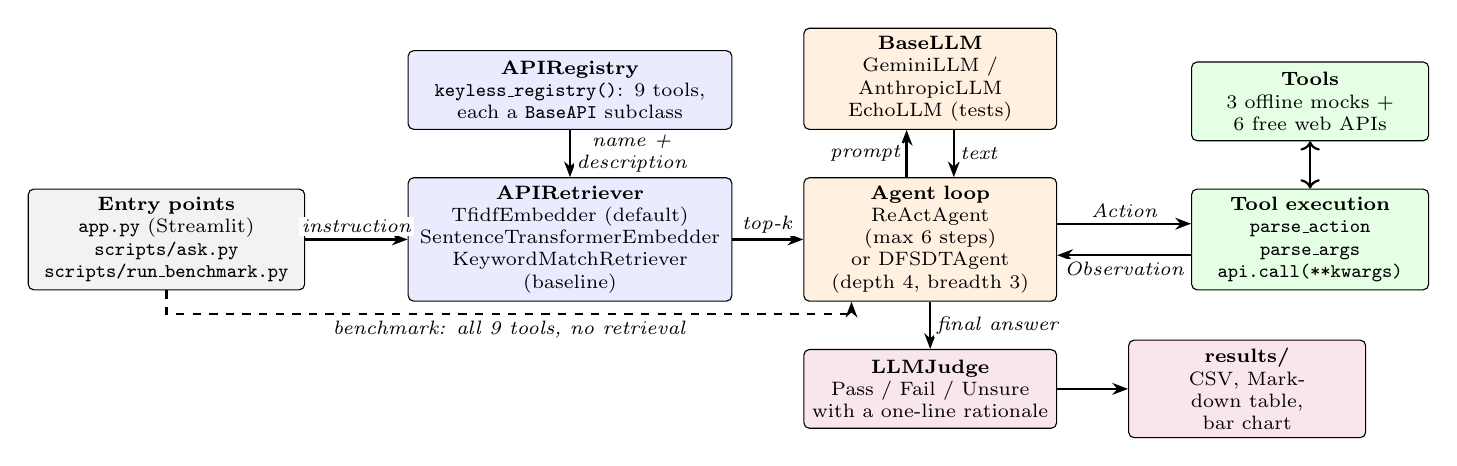
\begin{tikzpicture}[
    font=\scriptsize,
    box/.style={draw, rounded corners=2pt, align=center, minimum height=1.0cm, inner sep=3pt, fill=#1},
    box/.default=white,
    arr/.style={-{Stealth[length=2mm]}, thick},
    lbl/.style={font=\scriptsize\itshape, align=center, fill=white, inner sep=1pt},
    node distance=6mm and 9mm
  ]
  % entry points
  \node[box=gray!10, text width=3.3cm] (ui) {\textbf{Entry points}\\ \texttt{app.py} (Streamlit)\\ \texttt{scripts/ask.py}\\ \texttt{scripts/run\_benchmark.py}};

  % retrieval
  \node[box=blue!8, text width=3.9cm, right=13mm of ui] (ret) {\textbf{APIRetriever}\\ TfidfEmbedder (default)\\ SentenceTransformerEmbedder\\ KeywordMatchRetriever (baseline)};
  \node[box=blue!8, text width=3.9cm, above=of ret] (reg) {\textbf{APIRegistry}\\ \texttt{keyless\_registry()}: 9 tools,\\ each a \texttt{BaseAPI} subclass};

  % agents
  \node[box=orange!12, text width=3.0cm, right=of ret] (agent) {\textbf{Agent loop}\\ ReActAgent (max 6 steps)\\ or DFSDTAgent\\ (depth 4, breadth 3)};
  \node[box=orange!12, text width=3.0cm, above=of agent] (llm) {\textbf{BaseLLM}\\ GeminiLLM / AnthropicLLM\\ EchoLLM (tests)};

  % tools
  \node[box=green!10, text width=2.8cm, right=17mm of agent] (tools) {\textbf{Tool execution}\\ \texttt{parse\_action}\\ \texttt{parse\_args}\\ \texttt{api.call(**kwargs)}};
  \node[box=green!10, text width=2.8cm, above=of tools] (ext) {\textbf{Tools}\\ 3 offline mocks +\\ 6 free web APIs};

  % evaluation
  \node[box=purple!10, text width=3.0cm, below=of agent] (judge) {\textbf{LLMJudge}\\ Pass / Fail / Unsure\\ with a one-line rationale};
  \node[box=purple!10, text width=2.8cm, right=of judge] (res) {\textbf{results/}\\ CSV, Markdown table,\\ bar chart};

  \draw[arr] (ui) -- node[lbl, above=1pt] {instruction} (ret);
  \draw[arr] (reg) -- node[lbl, right=1pt] {name +\\description} (ret);
  \draw[arr] (ret) -- node[lbl, above=1pt] {top-$k$} (agent);
  \draw[arr] ([xshift=-3mm]agent.north) -- node[lbl, left=1pt] {prompt} ([xshift=-3mm]llm.south);
  \draw[arr] ([xshift=3mm]llm.south) -- node[lbl, right=1pt] {text} ([xshift=3mm]agent.north);
  \draw[arr] ([yshift=2mm]agent.east) -- node[lbl, above=1pt] {Action} ([yshift=2mm]tools.west);
  \draw[arr] ([yshift=-2mm]tools.west) -- node[lbl, below=1pt] {Observation} ([yshift=-2mm]agent.east);
  \draw[arr, <->] (tools) -- (ext);
  \draw[arr] (agent) -- node[lbl, right=1pt] {final answer} (judge);
  \draw[arr] (judge) -- (res);
  \draw[arr, dashed] (ui.south) -- ++(0,-3mm) -| node[lbl, pos=0.25, below=1pt] {benchmark: all 9 tools, no retrieval} ([xshift=-10mm]agent.south);
\end{tikzpicture}

  \caption{Architecture of ToolAgent. Boxes name the real classes and
  files. The dashed path marks a detail that is easy to miss: the
  benchmark script hands all nine keyless tools straight to the agents,
  so retrieval quality does not affect the benchmark numbers.}
  \label{fig:arch}
\end{figure*}

We kept three boundaries on purpose. Any \code{BaseAPI} can be registered
without touching the retriever or agents. Any \code{BaseLLM} can drive
either agent, which let us add Gemini later in one commit and lets the
tests run with no network. Any list of rows can be scored by the
\code{eval/} code. These boundaries paid off when we switched model
providers in the middle of the project.

\section{Implementation}

\subsection{Tool registry}
Every tool subclasses \code{BaseAPI} and declares a \code{name}, a one-line
\code{description}, a \code{parameters} dictionary and a \code{call()}
method that returns an \texttt{APIResponse(success, data, error)}. Tools
report errors in this object instead of raising, so the agent can show a
failure to the model as an observation.

There are three offline tools. \code{calculator} parses the expression
with Python's \code{ast} module and only allows numbers and the operators
\texttt{+ - * / ** \%} (and unary signs), so a model cannot run arbitrary code through
it. \code{weather} is a hard-coded table for Paris, Tokyo and New York, and
\code{search} matches words against four fixed sentences. The online
wrappers call Frankfurter for currency~\cite{frankfurter}, the Wikipedia
summary endpoint~\cite{wikipediarest}, the Free Dictionary
API~\cite{freedictionary}, JokeAPI~\cite{jokeapi}, Quotable~\cite{quotable},
REST Countries~\cite{restcountries}, OpenWeatherMap and NewsAPI.

\code{apis/registry.py} builds three registries: \code{default_registry()}
with the three mocks, \code{full_registry()} with all 11, and
\code{keyless_registry()} with the 9 tools that need no key of their own.
We added the keyless one so that the benchmark only needs a model key.

\subsection{Retriever}
\code{APIRetriever} joins each tool's name and description into one
string, fits an embedder on those strings, and ranks tools by cosine
similarity to the instruction. The embedder only needs \code{fit()} and
\code{similarity()}, so \code{TfidfEmbedder} and
\code{SentenceTransformerEmbedder} are interchangeable.
\code{KeywordMatchRetriever} is a separate baseline that scores by Jaccard
overlap of word sets. Both word-based methods share one tokenizer in
\code{retriever/text.py}, which lower-cases the text and strips a few
common suffixes (Section~\ref{sec:stem}). TF-IDF is the default because it
needs no model download.

\subsection{ReAct agent}
\code{ReActAgent.run()} loops up to \code{max_steps}~=~6 times. Each turn,
\code{build_prompt()} concatenates the instructions in
\code{REACT_SYSTEM_PROMPT}, the tool list, the user instruction and the
history so far, and sends it as one user message. The reply is first cut
at its first \texttt{Observation:} line, because only the tool may supply
observations. \code{parse_step()} then looks for \texttt{Action: name[args]}
and \code{Finish[...]}, and whichever comes first wins. If it is an
action, \code{parse_args()} turns the bracket text into keyword
arguments, the tool is called, and \texttt{Observation: ...} is added to the
history. Unknown tool names and exceptions become \code{Error:}
observations instead of crashing the run.

\subsection{DFSDT-inspired agent}\label{sec:dfsdt}
\code{DFSDTAgent} reuses the same prompt and parser but replaces the loop
with a recursive \code{_search()} (Fig.~\ref{fig:tree}). At each depth it
asks the model for up to \code{branching_factor}~=~3 replies. A reply that
finishes ends the search. A reply with an unparseable action, an unknown
tool, an exception or a failed \code{APIResponse} is dropped and the next
sibling is sampled. A reply with a successful call goes one level deeper
with the new observation in the history. If the whole subtree returns
nothing, the loop moves to the next sibling, which is the backtracking
step. Depth is capped at 4. The counter \code{explored_paths} records how
many replies were sampled.

\begin{figure}[t]
  \centering
  % How our DFSDTAgent._search walks the tree (drawn by us).
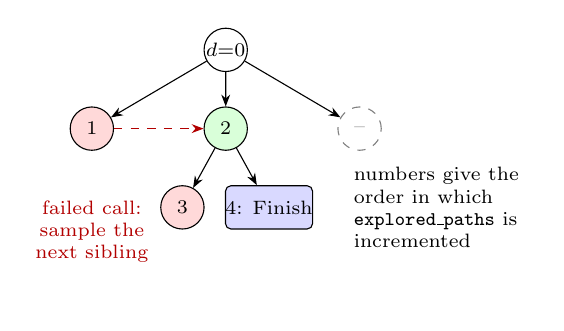
\begin{tikzpicture}[
    font=\scriptsize,
    every node/.style={draw, circle, minimum size=5.5mm, inner sep=0pt},
    ok/.style={fill=green!15},
    bad/.style={fill=red!15},
    fin/.style={fill=blue!15, rectangle, rounded corners=2pt, minimum width=8mm},
    level distance=10mm,
    level 1/.style={sibling distance=17mm},
    level 2/.style={sibling distance=11mm},
    edge from parent/.style={draw, -{Stealth[length=1.5mm]}}
  ]
  \node (root) {$d{=}0$}
    child { node[bad] (a) {1} }
    child { node[ok] (b) {2}
      child { node[bad] (c) {3} }
      child { node[fin] (d) {4: Finish} }
    }
    child { node[draw=gray, dashed, text=gray] {--} };
  \draw[-{Stealth[length=1.5mm]}, dashed, red!70!black]
    (a.east) -- (b.west);
  \node[draw=none, red!70!black, align=center, below=2mm of a] {failed call:\\ sample the\\ next sibling};
  \node[draw=none, anchor=west, text width=2.2cm, align=left] at ([xshift=4mm]d.east)
    {numbers give the order in which \texttt{explored\_paths} is incremented};
\end{tikzpicture}

  \caption{Order of exploration in \texttt{DFSDTAgent.\_search}. Node~1's
  tool call fails, so a sibling is sampled; node~2 succeeds and the
  search goes deeper. The third root branch is never sampled.}
  \label{fig:tree}
\end{figure}

We call this ``DFSDT-inspired'' because it differs from ToolLLM's version
in three ways. First, siblings are drawn by sending the exact same prompt
again, so variety comes only from sampling randomness; the failed sibling
is not shown to the model. ToolLLM's version, as we understand it, makes
the model aware of earlier attempts so it tries something new~\cite{qin2024toolllm}.
Second, our search has no explicit ``give up and restart'' action. Third,
a \code{Finish} reply is accepted without any check that it is supported
by observations.

\subsection{LLM layer}
All model access goes through \code{BaseLLM}, whose only method is
\code{generate(prompt)}. Two classes wrap the vendor SDKs
(\code{AnthropicLLM} and \code{GeminiLLM}), and \code{EchoLLM} replays a scripted list of replies for tests. The benchmark
and UI pick the back end from the \code{BENCHMARK_PROVIDER} variable in a
local \code{.env} file. The default is Gemini with
\code{gemini-3.5-flash-lite}~\cite{gemini}. Our \code{.env} sets only the
provider, so the benchmark ran with these defaults. \code{GeminiLLM} retries on HTTP 429, 500, 502, 503 and
504 with exponential backoff that starts at 2\,s and doubles, for up to 5
retries.

\subsection{Streamlit UI}
\code{app.py} has three tabs: \emph{Run Agent}, \emph{Compare ReAct vs
DFSDT} and \emph{Results Dashboard}. A sidebar selects the strategy and the
number of tools to retrieve (1 to 9, default 5). Unlike the benchmark, the
UI does use the TF-IDF retriever. Each run shows the candidate tools, the
final answer and a step-by-step trace that splits every reply into its
thought, action and observation, plus a badge when DFSDT explored more
branches than it kept. Registry and retriever are cached with
\code{st.cache_resource}, and \code{friendly_error()} turns rate-limit,
timeout and missing-key errors into short messages. The UI is built with
Streamlit~\cite{streamlit}.

\section{Evaluation Method and Results}

\subsection{Benchmark and procedure}
\code{data/benchmark_instructions.json} holds 19 instructions that we
wrote: 9 \emph{easy} (one tool), 6 \emph{medium} (two tools) and 4
\emph{hard} (three tools). The script \code{scripts/run_benchmark.py}
runs both agents on each one with all 9 keyless tools as candidates and
sends each
final answer to \code{LLMJudge.judge_pass()}, which replies \emph{Pass},
\emph{Fail} or \emph{Unsure} with a one-sentence rationale. Only
\emph{Pass} counts toward the pass rate. The judge uses the same model as
the agents. The script writes \code{benchmark_results.csv},
\code{comparison_table.md} and a bar chart. A win-rate comparator
(\code{LLMJudge.compare()}) is implemented and unit-tested but was not part
of this run.

\noindent\fbox{\parbox{\dimexpr\columnwidth-2\fboxsep-2\fboxrule}{\small
\textbf{Status note.} All benchmark numbers in this section are
\prov{}. They come from the run committed on 18~September~2026, before
our fixes. While reading the CSV we found that the agent loop accepted
tool results the model had made up (Section~\ref{sec:fake-obs}), so these
pass rates mostly measure the model's own knowledge rather than tool
use. The fixes are now in the code, but the benchmark has not been
re-run yet; corrected pass rates: \tbf{}.}}

\subsection{Provisional pass rates}
Table~\ref{tab:pass} and Fig.~\ref{fig:pass} give the judged pass rates.
Both agents failed bench-14, which asked for 50~USD in yen; both answered
7{,}500~yen and the judge marked it as a wrong rate. ReAct also failed
bench-03 (100~USD to euros), where it used all 6 steps without
finishing. DFSDT got \emph{Unsure} on bench-03 and bench-10 because the
judge could not check a live exchange rate.

\begin{table}[t]
  \centering
  \caption{\prov{} pass rates from \texttt{results/comparison\_table.md}}
  \label{tab:pass}
  \small
  \setlength{\tabcolsep}{4pt}
  \begin{tabular}{lccc}
    \toprule
    Complexity & ReAct & DFSDT-insp. & $N$ \\
    \midrule
    Easy    & 89\% (8/9)   & 89\% (8/9)   & 9 \\
    Medium  & 83\% (5/6)   & 67\% (4/6)   & 6 \\
    Hard    & 100\% (4/4)  & 100\% (4/4)  & 4 \\
    \midrule
    Overall & 89\% (17/19) & 84\% (16/19) & 19 \\
    \midrule
    \multicolumn{4}{l}{Win rate, DFSDT vs ReAct: \tbf{}} \\
    \bottomrule
  \end{tabular}
\end{table}

\begin{figure}[t]
  \centering
  % Provisional pass rates from results/comparison_table.md (run of 18 Sep 2026).
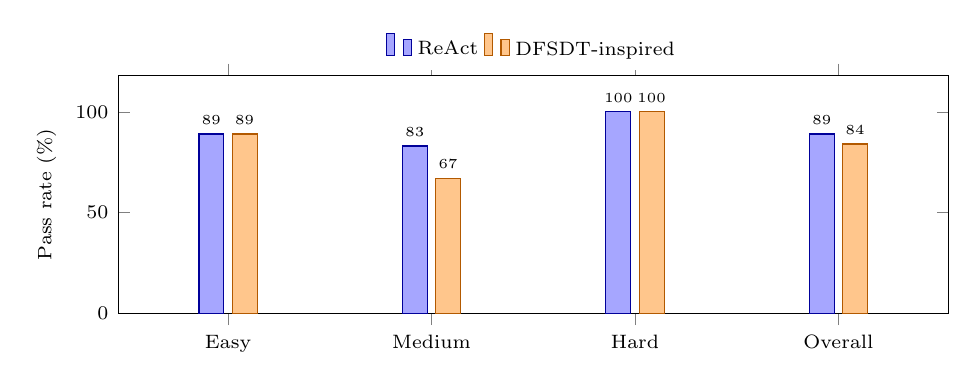
\begin{tikzpicture}
  \begin{axis}[
      ybar=3pt,
      width=\columnwidth,
      height=4.6cm,
      bar width=9pt,
      ymin=0, ymax=118,
      ylabel={Pass rate (\%)},
      symbolic x coords={Easy,Medium,Hard,Overall},
      xtick=data,
      nodes near coords,
      every node near coord/.append style={font=\tiny},
      tick label style={font=\scriptsize},
      label style={font=\scriptsize},
      legend style={font=\scriptsize, at={(0.5,1.02)}, anchor=south, legend columns=2, draw=none},
      enlarge x limits=0.18,
    ]
    \addplot[fill=blue!35, draw=blue!60!black] coordinates {(Easy,89) (Medium,83) (Hard,100) (Overall,89)};
    \addplot[fill=orange!45, draw=orange!70!black] coordinates {(Easy,89) (Medium,67) (Hard,100) (Overall,84)};
    \legend{ReAct, DFSDT-inspired}
  \end{axis}
\end{tikzpicture}

  \caption{Provisional pass rate by instruction complexity, redrawn from our
  own \texttt{results/comparison\_table.md}.}
  \label{fig:pass}
\end{figure}

\subsection{Why we do not trust these numbers yet}\label{sec:distrust}
The \code{react_steps} and \code{dfsdt_steps} columns are 1 in 37 of the
38 runs. A three-tool question cannot be solved honestly in one step. The
answers also disagree with our own mock tools. The \code{weather} tool
returns ``Cloudy, 18\,\textdegree C'' for Paris and ``Clear,
27\,\textdegree C'' for Tokyo, but the agents reported 15\,\textdegree C
and partly cloudy for Paris (bench-02) and 18\,\textdegree C and partly
cloudy for Tokyo (bench-11). The judge passed all of these because it
never saw the tool output. Hard tasks scoring 100\% is therefore a sign of
the bug, not of skill.

\subsection{Retriever check}
Because the benchmark skips retrieval, we measured the retrievers on their
own. For each benchmark instruction we ranked the 9 keyless tools and
checked the top~3, before and after the tokenizer fix of
Section~\ref{sec:stem} (Table~\ref{tab:ret}). This needs no model calls,
so these numbers are final.

\begin{table}[t]
  \centering
  \caption{Retrievers on the 19 benchmark instructions (9 tools)}
  \label{tab:ret}
  \small
  \setlength{\tabcolsep}{4pt}
  \begin{tabular}{lccc}
    \toprule
    Retriever & Top-1 & All needed & Top score \\
              & correct & in top 3 & is 0.0 \\
    \midrule
    Keyword, before fix & 12 & 11 & 2 \\
    TF-IDF, before fix  & 12 & 11 & 2 \\
    Keyword, after fix  & 15 & 14 & 0 \\
    TF-IDF, after fix   & 15 & 14 & 0 \\
    MiniLM embeddings   & 17 & 17 & 0 \\
    \bottomrule
  \end{tabular}
\end{table}

Before the fix, on ``Convert 100 US dollars to Euros.'' both word-based
retrievers gave every tool 0.0, while MiniLM ranked
\code{currency_exchange} first with 0.601. After the fix, TF-IDF ranks
it first with 0.386. The semantic retriever is still the best of the
three.

\section{Challenges and Lessons Learned}

\subsection{The loop accepted made-up tool results}\label{sec:fake-obs}
Our prompt shows the model the full pattern \texttt{Thought / Action /
Observation / ... / Finish[...]}, and we call the model with no stop
sequence. The model therefore often writes an action, then a fake
observation, then \code{Finish[...]} in one reply. \code{ReActAgent}
checked for \code{Finish} before it checked for an action, so it returned
the final answer and never called the tool. \code{DFSDTAgent} did the same.
The evidence is in Section~\ref{sec:distrust}. Our unit tests did not catch it because
every scripted \code{EchoLLM} reply contains only one action or one
finish.

We fixed it in three places. In \code{agent/parsing.py}, the new function
\code{truncate_at_observation()} drops everything from the first
\texttt{Observation:} line of a reply, so a guessed result and the
\code{Finish} after it never reach the agent or the history.
\code{parse_step()} returns whichever of \code{Action} and \code{Finish}
comes first, so an action written before a guessed answer is run. Both
agents use these two functions. Finally, the prompt now tells the model
to write one action, stop, and never write an observation itself. New
tests script exactly the bad reply we saw, \texttt{Action:
calculator[23 * 17]}, a fake \texttt{Observation: 400} and
\code{Finish[400]}, and check that both agents run the calculator and
answer 391.

\subsection{Argument parsing}\label{sec:args}
We found three problems in \code{agent/parsing.py}, all reproduced
offline, and fixed each one:
\begin{enumerate}\raggedright
  \item \code{ACTION_PATTERN} uses a greedy \texttt{(.*)\textbackslash]}
        with \code{DOTALL}, so on a multi-part reply the arguments run to
        the last \code{]}. For \texttt{calculator[23 * 17]} followed by a
        fake observation and \code{Finish[391]}, the captured argument was
        \texttt{23 * 17]\textbackslash nObservation: 391\textbackslash nFinish[391}.
        \emph{Fix:} the pattern now stops at the end of the line, so the
        argument is \texttt{23 * 17}.
  \item \code{parse_args()} splits on every comma. The documented
        OpenWeatherMap form \code{city=London,GB} becomes
        \texttt{\{\textquotesingle{}city\textquotesingle{}: \textquotesingle{}London\textquotesingle{}, \textquotesingle{}GB\textquotesingle{}: \textquotesingle{}\textquotesingle{}\}}, and positional
        \texttt{USD, EUR, 100} is passed whole as \code{base}.
        \emph{Fix:} keyword arguments are split only at a comma that
        starts a new \texttt{key=}, and positional values are mapped onto
        the parameters in order, but only for tools that need more than
        one argument (found with \code{inspect.signature}).
  \item All values stay strings. A well-formed
        \texttt{currency\_exchange[base=USD, target=EUR, amount=100]}
        always fails, because \code{CurrencyExchangeAPI.call()} divides a
        float by \texttt{\textquotesingle{}100\textquotesingle{}}. With a mocked HTTP response the observation
        was \texttt{Error: unsupported operand type(s) for /: \textquotesingle{}float\textquotesingle{} and
        \textquotesingle{}str\textquotesingle{}}. This fits ReAct's six-step failure on bench-03, though we
        did not save that trace and cannot confirm it. \emph{Fix:}
        \code{currency_exchange} is our only tool with a numeric
        parameter, so it now converts \code{amount} itself and returns
        a clear error for text such as ``a lot''. We did not add type
        guessing to the parser, because the calculator needs its
        expression as text.
\end{enumerate}
An earlier and related bug is fixed. When a model left out a required
argument, \code{api.call(**kwargs)} raised \code{TypeError} and the whole
run crashed. Commit \code{495b278} wrapped the call: ReAct now records an
\code{Error:} observation and DFSDT treats the branch as failed. Two tests
cover this. The three fixes above have their own tests in
\code{tests/test_parsing.py}, \code{tests/test_agent.py} and
\code{tests/test_external_apis.py}.

\subsection{Retriever scored 0.0 on unstemmed words}\label{sec:stem}
Both word-based retrievers compare exact lower-case tokens. The
\code{currency_exchange} description says ``Converts \ldots{} currencies'',
but users write ``convert'' and ``dollars''. With no shared token, the
keyword and TF-IDF scores were 0.0 for every tool, so the top~3 was just
registry order (calculator, weather, search). The same happened for bench-01, ``What is 23 times 17?'', because the
\code{calculator} description never uses the word ``times''.

We fixed this in two ways. First, \code{retriever/text.py} adds a very
small suffix stripper, much simpler than the Porter
stemmer~\cite{porter1980}: it maps ``ies'' to ``y'' and removes ``ing'',
``ed'' and a final ``s'', leaving short words and endings such as ``us''
alone. TF-IDF and the keyword baseline both use it, so ``converts'' and
``convert'' now match. Second, we added the words people actually type to
two descriptions: ``multiply or times'' for the calculator and ``money
(e.g.\ dollars, euros, yen)'' for currency. Table~\ref{tab:ret} shows the
effect: no instruction scores 0.0 any more. We kept TF-IDF as the UI
default to avoid the model download.

\subsection{Free-tier rate limits}
A benchmark pass makes at least four model calls per instruction (one
for each agent and one judge call for each answer), and DFSDT can make up
to 3 calls per level. On a free Gemini key this ran into HTTP 429 errors.
We added the retry loop in \code{GeminiLLM} and the friendly 429 message
in the UI. We have not yet measured how long a full benchmark run
takes: \tbf{}.

\subsection{Slow install}
Installing \code{sentence-transformers} also installs PyTorch, which
makes the \code{requirements.txt} install by far the slowest setup step. We kept TF-IDF as the
default, and \code{SentenceTransformerEmbedder} imports the library inside
\code{__init__} so that importing the retriever package stays light.
Our finished virtual environment (PyTorch 2.14.0 CPU build,
sentence-transformers 6.0.1, Streamlit 1.64.0) takes 1.6\,GB on disk.
We did not time a clean install: \tbf{}.

\subsection{Model-agnostic code paid off}
We started on the Anthropic API and later moved the benchmark to
Gemini. Because both agents only see \code{BaseLLM}, the switch was
one new 63-line class and one environment variable.

\section{Testing}
The \code{tests/} folder has 72 tests in 8 files, and all 72 pass
(\code{pytest}, about 18\,s on our machine). Agent tests use \code{EchoLLM} to script the model: one checks
that ReAct calls the calculator and finishes with 89; another checks that
DFSDT backtracks past a failing \code{weather[city=Atlantis]} call and
reports \code{explored_paths}~=~3. The eight web-API wrappers are tested
with \code{unittest.mock.patch} on \code{requests.get}, so the suite needs
no network. The judge tests feed scripted judge replies, including
malformed ones, to check verdict parsing. The semantic retriever test
skips itself if \code{sentence-transformers} is missing.

Our first 52 tests assumed the model behaves, with one action per reply,
which is why they missed the bug in Section~\ref{sec:fake-obs}. We added
20 tests for the fixes: fake observations and an action followed by a
guessed \code{Finish} (for both agents), the parsing cases of
Section~\ref{sec:args}, text and non-numeric amounts for currency, and
the unstemmed queries of Section~\ref{sec:stem} for both word-based
retrievers. To check that these tests really catch the bugs, we ran them
against the code from before the fixes: 11 of them failed there, and the
new parser tests could not even be imported. All of them pass on the fixed
code.

\section{Limitations}\label{sec:limits}
\begin{itemize}
  \item The benchmark results are \prov{}: they predate the fixes and
        have not been re-run.
  \item 19 instructions written by us is a very small test set, and we
        wrote them knowing which tools exist.
  \item The judge is the same model as the agents and only sees the final
        answer, not the tool outputs. Self-preference is a known judge
        bias~\cite{zheng2023judge}. Questions about live exchange rates
        cannot be checked by the judge at all.
  \item Three of our tools are mocks with tiny data (three cities, four
        sentences).
  \item The benchmark does not use the retriever, so the end-to-end
        pipeline that the UI runs has not been scored.
  \item The harness saves only answers and step counts, not full traces.
\end{itemize}

\section{Future Work}
\begin{enumerate}
  \item Re-run the benchmark on the fixed code and replace every
        \prov{} value.
  \item Save the full step trace of every run as JSON next to the CSV.
  \item Give the judge the observations, use a different model as judge,
        and run the win-rate comparison.
  \item Show failed siblings to the model in \code{DFSDTAgent} so retries
        differ, closer to ToolLLM's DFSDT.
  \item Run the benchmark through the retriever with a smaller $k$, and
        add instructions where several tools look relevant.
\end{enumerate}

\section{Conclusion}
We built a working small-scale version of the ToolLLM pipeline: tool
wrappers, three retrievers, a ReAct agent, a DFSDT-inspired search agent,
an LLM judge and a UI, with 72 passing tests. The most useful thing we
learned came from reading our own results: a high pass rate meant little
once we saw that the model was writing its own observations. Our first
numbers (89\% for ReAct, 84\% for DFSDT) are therefore \prov{}. We have
fixed that bug, the three parsing bugs and the retriever's exact-match
problem, each with tests. The retriever comparison needed no model and is
final: a needed tool now comes first for 15 of 19 instructions with
TF-IDF (12 before the fix) and 17 of 19 with sentence embeddings. Phase~2
starts with a clean re-run of the benchmark.

\bibliographystyle{IEEEtran}
{\raggedright
\bibliography{references}
}

\appendices
\section{Sample Trace}
Our harness does not store intermediate steps, so the most detailed
record we have is one CSV row. Below is the ReAct row for bench-11 from
\code{results/benchmark_results.csv}, exactly as saved (answer and
rationale fields wrapped for width):

\begin{lstlisting}
id:          bench-11  (medium)
instruction: What's the weather in Tokyo, and what is
             the population of Japan?
expected:    weather;country_info
react_steps: 1
answer:      The weather in Tokyo is 18°C and partly
             cloudy, and the population of Japan is
             125,800,000.
verdict:     pass
rationale:   The agent's final answer successfully
             provides both the current weather in Tokyo
             and the population of Japan as requested.
\end{lstlisting}

For comparison, this is what our \code{weather} tool actually returns
for Tokyo when called directly:

\begin{lstlisting}
>>> WeatherAPI().call(city='Tokyo')
APIResponse(success=True,
  data={'condition': 'Clear', 'temperature_c': 27},
  error=None)
\end{lstlisting}

The step count of 1 and the mismatched weather show the made-up
observation problem in one example. A full Thought / Action / Observation
trace from the corrected agent will be added here: \tbf{}.

\end{document}
